\begin{figure}[htb]
\subfloat[]{\makebox[.5\textwidth]{
\begin{tikzpicture}[scale = 10]
\tikzstyle{VertexStyle} = []
\tikzstyle{EdgeStyle} = []
\tikzstyle{labeledStyle}=[shape = circle, minimum size = 6pt, inner sep = 1.2pt, draw]
\tikzstyle{unlabeledStyle}=[shape = circle, minimum size = 6pt, inner sep = 1.2pt, draw, fill]
\Vertex[style = labeledStyle, x = 0.5, y = 0.899999998509884, L = \tiny {$0, 6, 7$}]{v0}
\Vertex[style = labeledStyle, x = 0.349999994039536, y = 0.799999997019768, L = \tiny {$1, 3, 6$}]{v1}
\Vertex[style = labeledStyle, x = 0.649999976158142, y = 0.799999997019768, L = \tiny {$2, 3, 7$}]{v2}
\Vertex[style = labeledStyle, x = 0.400000005960464, y = 0.650000005960464, L = \tiny {$4, 6, 7$}]{v3}
\Vertex[style = labeledStyle, x = 0.600000023841858, y = 0.650000005960464, L = \tiny {$5, 6, 7$}]{v4}
\Edge[label = \tiny {}, labelstyle={auto=right, fill=none}](v1)(v0)
\Edge[label = \tiny {}, labelstyle={auto=right, fill=none}](v2)(v0)
\Edge[label = \tiny {}, labelstyle={auto=right, fill=none}](v2)(v4)
\Edge[label = \tiny {}, labelstyle={auto=right, fill=none}](v3)(v1)
\Edge[label = \tiny {}, labelstyle={auto=right, fill=none}](v3)(v4)
\end{tikzpicture}
}}
\subfloat[]{\makebox[.5\textwidth]{
\begin{tikzpicture}[scale = 10]
\tikzstyle{VertexStyle} = []
\tikzstyle{EdgeStyle} = []
\tikzstyle{labeledStyle}=[shape = circle, minimum size = 6pt, inner sep = 1.2pt, draw]
\tikzstyle{unlabeledStyle}=[shape = circle, minimum size = 6pt, inner sep = 1.2pt, draw, fill]
\Vertex[style = labeledStyle, x = 0.400000005960464, y = 0.899999998509884, L = \tiny {$0, 1, 11, 12$}]{v0}
\Vertex[style = labeledStyle, x = 0.25, y = 0.799999997019768, L = \tiny {$2, 3, 6, 11$}]{v1}
\Vertex[style = labeledStyle, x = 0.550000011920929, y = 0.799999997019768, L = \tiny {$4, 5, 6, 12$}]{v2}
\Vertex[style = labeledStyle, x = 0.300000011920929, y = 0.650000005960464, L = \tiny {$7, 8, 11, 12$}]{v3}
\Vertex[style = labeledStyle, x = 0.5, y = 0.650000005960464, L = \tiny {$9, 10, 11, 12$}]{v4}
\Edge[label = \tiny {}, labelstyle={auto=right, fill=none}](v1)(v0)
\Edge[label = \tiny {}, labelstyle={auto=right, fill=none}](v2)(v0)
\Edge[label = \tiny {}, labelstyle={auto=right, fill=none}](v2)(v4)
\Edge[label = \tiny {}, labelstyle={auto=right, fill=none}](v3)(v1)
\Edge[label = \tiny {}, labelstyle={auto=right, fill=none}](v3)(v4)
\end{tikzpicture}
}}
\caption{
Counterexamples to Conjecture \ref{MoonshineConjecture}.
}
\label{fig:goldbergce}
\end{figure}
